\documentclass[12pt]{scrartcl}

% packages

% \usepackage{blindtext}

\usepackage[utf8]{inputenc}
\usepackage[T1]{fontenc}
\usepackage[english]{babel}

\usepackage[top=30mm, bottom=30mm, left=20mm, right=20mm]{geometry}
\usepackage{fancyhdr}
\usepackage{setspace}
\usepackage{parskip}

\usepackage{graphicx}
\usepackage[section]{placeins}
\usepackage[table, dvipsnames]{xcolor}
\usepackage{pdfpages}

\usepackage{hyperref}
\usepackage[labelfont=bf]{caption}

\usepackage[round]{natbib}

\usepackage{listings}
\usepackage{minted}
\usepackage{algorithmicx}
\usepackage[noend]{algpseudocode}
\usepackage{algorithm}

\usepackage{tabularx}
\usepackage{multirow}
\usepackage{multicol}
\usepackage{caption}
\usepackage{subcaption}
\usepackage{adjustbox}

\usepackage{amsmath}

%%%%%%%%%%%%%%%%%%%%%% preamble %%%%%%%%%%%%%%%%%%%%%%

\renewcommand*{\sectionmark}[1]{ \markright{\thesection\ ##1} }
% \renewcommand*{\chaptermark}[1]{ \markboth{\chaptername\ \thechapter: ##1}{} }
\fancyhead[LE,RO]{\thepage}
\fancyhead[LO,RE]{}
\fancyfoot{}
\pagestyle{fancy}

\definecolor{myblue}{RGB}{46, 59, 160}

\graphicspath{{pics/}}

\hypersetup{
	pdfstartpage=7,
    pdfstartview = FitB,
	pdfpagelayout=SinglePage,
	pdftitle={Project Report},
	pdfsubject={Statistical Learning Theory},
	pdfauthor={Maurice Wenig},
	pdfcreator={Maurice Wenig},
	pdfproducer={Maurice Wenig},
	pdfkeywords={meta, information, pdf, hyperref, latex},
	colorlinks=true,
	linkcolor=myblue,
	citecolor=myblue
}

\bibliographystyle{unsrtnat}

\newcommand*\justify{%
  \hyphenchar\font=`\-% allowing hyphenation
}

\definecolor{line_number_colour}{rgb}{0.5,0.5,0.5}
\renewcommand\theFancyVerbLine{\color{line_number_colour}\tiny\arabic{FancyVerbLine}}
\setminted[C]{
	% linenos, 
	breaklines,
	fontsize=\footnotesize
}

\hyphenpenalty=5000
\tolerance=5000

% TODO: remove for digital version
% \selectcolormodel{gray}

%----- new commands
\newcommand{\Romannumeral}[1]{\MakeUppercase{\romannumeral #1}}
\newcommand{\set}[1]{\{#1\}}
\newcommand{\abs}[1]{\left\vert #1 \right\vert}
\newcommand{\norm}[1]{\left\| #1 \right\|}
\newcommand{\skal}[2]{\left\langle #1 | #2 \right\rangle}
\newcommand{\script}[1]{
    skripte/aufgabe#1.py
    \lstinputlisting{skripte/aufgabe#1.py}
}
%----- defs
\def\notiff{\mathrel{{\ooalign{\hidewidth$\not\phantom{"}$\hidewidth\cr$\iff$}}}}
\def\R{\mathbb{R}}
\def\bbone{\text{\usefont{U}{bbold}{m}{n}1}}
\def\1{\mathbb{1}}
\def\T{\top}
\def\ndy{
    \textcolor{red} {\hfill not done yet!}
    \reversemarginpar
    \marginpar{\raggedleft\textcolor{red}{\rule{2mm}{2mm}}}
}
\def\ghostline{\hfill\vspace*{-5mm}}

%%%%%%%%%%%%%%%%%%%%%% main %%%%%%%%%%%%%%%%%%%%%%

\begin{document}

\thispagestyle{empty}
\begin{center}
	\begin{LARGE}
		\textbf{Statistical Learning Theory LAB}
	\end{LARGE}\vspace{3mm}\\
	\begin{Large}
		\textbf{Project Report}
	\end{Large}\vspace{5mm}\\
	\begin{large}
		Maurice Wenig
	\end{large}
\end{center}
% \setcounter{tocdepth}{1}
\tableofcontents
\clearpage

% algorithm, its performance, technical details, your score
% In the report focus on the key features of your system.
% Especially if you do not implement the used algorithms yourself make sure to cover them in the report so its clear you could have implemented them yourself
% (i.e. someone could implement the algorithm only reading your report).
% If you combine several predictors, you should describe at least two of them in detail, for the others the basics should be enough.

\fancyhead[LO,RE]{\itshape\nouppercase\leftmark}
\section{Algorithms}
\subsection[Neighbourhood]{Neighbourhood-Based Recommenders}
\subsubsection[User-Based]{User-Based Recommender}
% include long tail plot
The user-based recommender compares users based on their rated items. An item rating from a user is then predicted based on ratings of that item from similar users.
The similarity measure used to compare users is Pearson:
$$\text{Sim}(u, v) = \frac{\sum\limits_{i\in I_{uv}} w_i \cdot s_{ui} s_{vi}}{\sqrt{\sum\limits_{i\in I_{uv}} w_i \cdot  s_{ui}} \cdot \sqrt{\sum\limits_{i\in I_{uv}} w_i \cdot  z_{vi}}}$$
where $I_{uv}$ are the items that both users $u$ and $v$ have rated, $s_{ui} = r_{ui} - \mu_u$ is the centered rating from user $u$.
The mean rating $\mu_u$ can be calculated individually for every comparison, based on only the common items, or it can be calculated once for every user, based on all their rated items.
$w_i = \log\frac{\text{\# users}}{\text{\# users who rated } i}$ are item weights to combat the impact of the long tail in the number of item ratings.
To prefer users with more common items, the similarites of users with less than $\beta$ common items are made smaller.
$$\text{Sim}(u, v) \gets \text{Sim}(u, v) \cdot \frac{\min\set{\abs{I_{uv}}, \beta}}{\beta}$$

Based on these similarities, a peer group $P_u(i)$ of users can be determined. For this, the users are sorted by similarity.
To improve efficiency in the online phase, the sorting is done in the offline phase.
In the online phase, this order is simply applied. Users who have not rated the item $i$ and users whos similarity does not exceed a certain threshold, are then removed.
The top $k$ remaining users are then the peer group $P_u(i)$.

The predicted item rating from a user is then calculated as a sum of ratings from similar users, weighted with their relative similarity.
The means and variances of the user ratings are normalized to not influence the prediction.
$$\hat{r}_{ui} = \mu_u + \sigma_u \cdot \frac{\sum\limits_{v \in P_u(i)} \text{Sim}(u, v) \cdot z_{vi}}{\sum\limits_{v \in P_u(i)} \abs{\text{Sim}(u, v)}}$$
where $z_{ui} = s_{ui} / \sigma_u$ is the normalized rating, $\sigma_u$ the variance of the ratings of user $u$.
If the user has only ever given one distinct rating, the variance is set to an arbitrary value of 1.

In special cases where the user or the item has never been seen before, similarities can not be calculated. In those special cases, the ratings were predicted in a different way:

\begin{itemize}
	\item user and item unknown: predict average between minimum and maximum possible rating
	\item user unknown, item known: predict average rating of that item
	\item user known, item unknown: predict average rating of that user
\end{itemize}

\subsubsection[Item-Based]{Item-Based Recommender}
The item-based recommender compares items based on their user ratings. An item rating from a user is then predicted based on ratings of similar items from that user.
It functions very similar to the user-based recommender. The similarity function is adapted to still use user means $\mu_u$ instead of item means $\mu_i$ to normalize user preferences.
The predicted rating is then a weighted sum of similar items, the user has rated.

$$\hat{r}_{ui} = \frac{\sum\limits_{j \in P_i(u)} \text{Sim}(i, j) \cdot r_{uj}}{\sum\limits_{j \in P_i(u)} \abs{\text{Sim}(i, j)}}$$

\subsubsection{Clustering}
To increase efficiency, the users/items can be clustered before the creation of the similarity matrix. This way, only users/items that are in the same cluster have to be compared.

This is done using an adapted version of K-means.
To account for the sparsity of the rankings matrix, the entries of the mean of a cluster are calculated using only vectors, where the entries are not missing in the respective dimensions.
The distance measure is also adapted. The distance between two vectors is calculated only with the common dimensions, where ratings are not missing.
The result is then divided by the number of common dimensions to get a distance measure that is independent of the number of common dimensions.


\subsection[Factorization]{Factorization-Based Recommender}
% include plot: didn't improve much from equally distributed weights


\subsection[Hybrid]{Hybrid Recommender}
bruh

\section{Results}
% also talk about hyper parameters
\subsection{Performance}
\subsection{Error Scores}
\subsection{Final Score}



% \section{Vorgehen}
% Das initiale Feld wird gleichmäßig auf alle Prozesse aufgeteilt. In jedem Prozess werden die neuen Temperaturen im lokalen $chunk$ berechnet. Dafür gibt es einen Austausch der aktuellen Werte mit den Nachbarprozessen. Diese Werte werden in den Ghost Cells in einem Halo der Breite $g$ um den lokalen $chunk$ gespeichert.
% Ab hier werden die Ghost Cells als Teil des lokalen Chunks angesehen. Der Teil des Chunks, der keine Ghost Cells beinhaltet, wird als innerer Chunk bezeichnet.
% Am Ende der Berechnung werden die innneren Chunks der einzelnen Prozesse wieder zusammengesetzt.

% \begin{algorithmic}[1]
%     \State split\_up\_domain()
%     \For{$i = 0 \rightarrow n\_iterations$}
%         \If{$i \% g == 0$}
%             \State exchange\_ghost\_cells()
%         \EndIf
%         \State calculate()
%     \EndFor
%     \State collect()
% \end{algorithmic}
% \subsection{Kommunikation}
% Die angewandten Techniken werden größtenteils dem Paper ``Ghost Cell Pattern'' von \citeauthor{Kjolstad2010} entnommen.
% Es wird ein Deep Halo benutzt und die Corner Cells sollen auch effizient übertragen werden.
% Da die Ost-West-Kommunikation immer vor der Nord-Süd-Kommunikation passieren muss, damit die Ecken richtig übertragen werden, wird zwischen der Kommunikation von den beiden Richtungen gewartet.

% \begin{algorithmic}[1]
%     \State irecv\_east()
%     \State irecv\_west()
%     \State isend\_east()
%     \State isend\_west()
%     \State wait()
%     \State irecv\_north()
%     \State irecv\_south()
%     \State isend\_north()
%     \State isend\_south()
%     \State wait()
% \end{algorithmic}

% Falls ein Nachbar in eine Richtung nicht existiert, werden die Ghost Cells mit Padding gefüllt. Dabei wird immer der nächste Wert des inneren Chunks kopiert.

% \subsection{Berechnung}
% Es werden immer nur so viele Zellen berechnet, wie für den nächsten Schritt benötigt werden. Dafür wird eine $border$ eingeführt.
% Am Anfang umfasst die $border$ den ganzen Chunk, inklusive Halo, bis auf den äußersten Ring. Am Ende umfasst die $border$ nur noch den inneren Chunk.
% % TODO: fancy visualisation

% Um die neuen Werte zu berechnen werden zwei Arrays benutzt. Eines, das die alten Werte enthält und eines, das die Ergebnisse der Berechnung enthält. Als Vorbereitung für den nächsten Schritt werden am Ende der Berechnung die Arrays vertauscht.

% \begin{algorithmic}[1]
%     \State $border$ := adapt\_border()
%     \For{$x,y$ in the $border$}
%         \State results[$x,y$] := calculation\_step($x,y$) \Comment{calculation\_step uses old\_values}
%     \EndFor
%     \State swap(results, old\_values)
% \end{algorithmic}


% \clearpage
% \section{Implementierung}
% % TODO: update lines
% \subsection{Chunks}
% Zu dem inneren Chunk kommt noch das Ghost-Block-Halo dazu:

% \subsection{Kommunikation}

% \subsection{Berechnung}
% Berechnung nach Aufgabenstellung mit \verb+FACTOR+ $= \alpha \cdot \frac{\Delta t}{h^2}$.


% \clearpage
% \section{Benutzung}
% Argumente, die übergeben werden müssen:
% \begin{itemize}
%     \item Größe des zu berechnenden Feldes
%     \item Anzahl der Iterationen
%     \item Anzahl der Prozesse in X-Richtung
%     \item Anzahl der Prozesse in Y-Richtung
% \end{itemize}
% Parameter, die angepasst werden können:
% \begin{itemize}
%     \item Ausgabedatei
%     \item Breite des Ghost Cell Halos
%     \item Abstand der Iterationen, in denen ein Zwischenstand gespeichert wird
% \end{itemize}

% \clearpage
% \section{Auswertung}
% (Disclaimer:) Die Performance wurde auf meinem lokalen Rechner gemessen, da es auf dem ARA-Cluster zu fehlern kam (siehe \verb+README.md+).

% \begin{figure}[!htb]
%     \begin{subfigure}{0.5\textwidth}
%         \centering
%         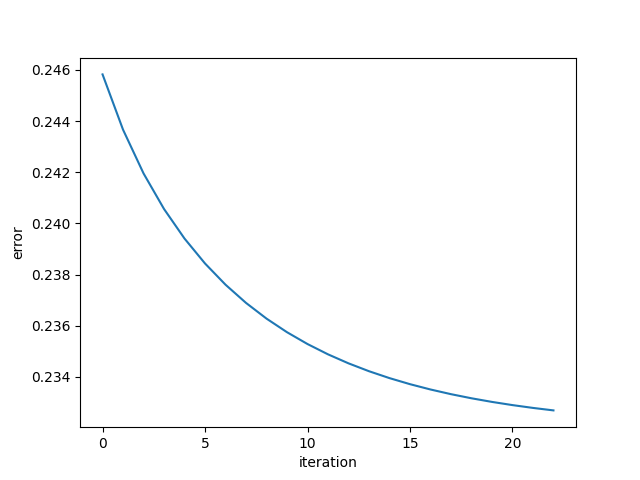
\includegraphics[scale=0.5]{../plots/descent.png}
%         \caption{field size 128}\label{fig:plot_128_tot}
%     \end{subfigure}
% 	\begin{subfigure}{0.5\textwidth}
%         \centering
%         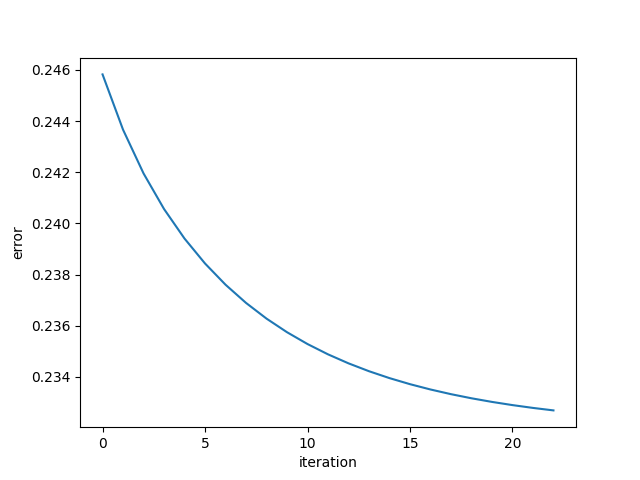
\includegraphics[scale=0.5]{../plots/descent.png}
%         \caption{field size 256}\label{fig:plot_256_tot}
%     \end{subfigure}
%     \newline
%     \begin{subfigure}{0.5\textwidth}
%         \centering
%         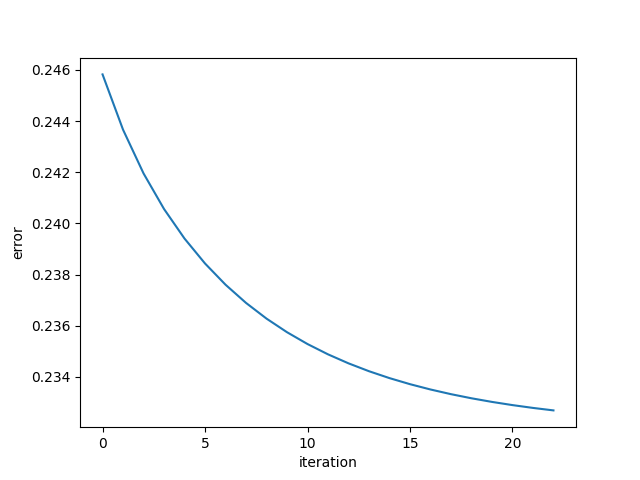
\includegraphics[scale=0.5]{../plots/descent.png}
%         \caption{field size 512}\label{fig:plot_512_tot}
%     \end{subfigure}
% 	\begin{subfigure}{0.5\textwidth}
%         \centering
%         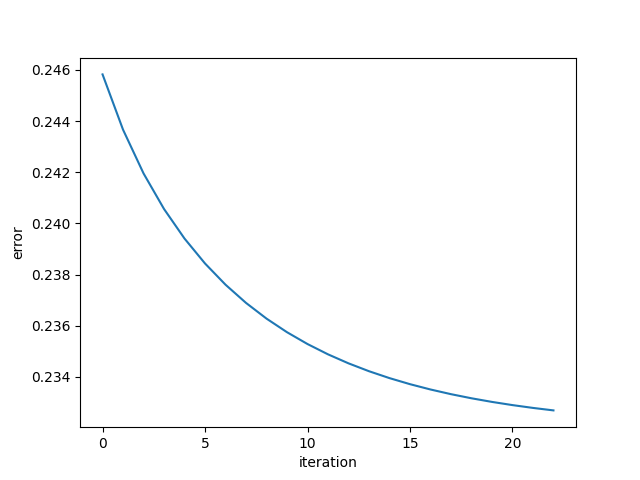
\includegraphics[scale=0.5]{../plots/descent.png}
%         \caption{field size 1024}\label{fig:plot_1024_tot}
%     \end{subfigure}
%     \begin{center}
%         \begin{subfigure}{0.5\textwidth}
%             \centering
%             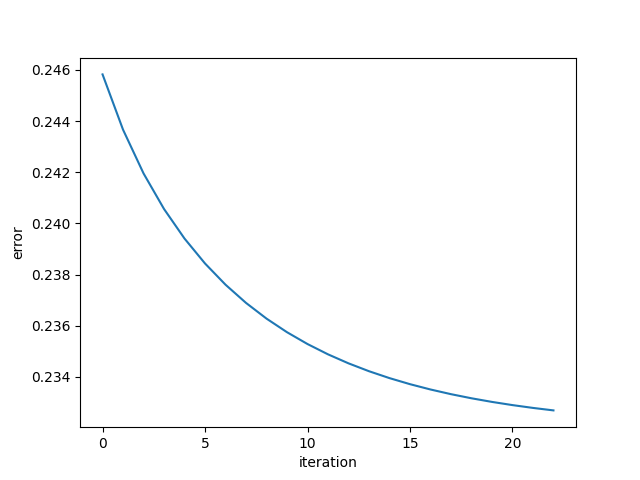
\includegraphics[scale=0.5]{../plots/descent.png}
%             \caption{field size 2048}\label{fig:plot_2048_tot}
%         \end{subfigure}
%     \end{center}
% 	\caption{Zeitverteilung gesamt}
%     \label{fig:all_time}
% \end{figure}

% Jeder Prozess hat einzeln die Zeiten der Berechnungs- und Kommunikationszeiten für einzelne Schritte gemessen. Daraus wurden Gesamtzeiten und Durchschnittszeiten der einzelnen Prozesse berechnet. Über den Prozessen wurde dann der Durchschnitt gezogen.
% Die Gesamtzeit des Programms wurde nur vom main rank gemessen.

% Wie man in \autoref{fig:all_time} sieht, führt eine Erhöhung der Halobreite zuerst zu einer Verbesserung der Laufzeit, da der Aufbau der Kommunikation deutlich länger braucht als die Berechnung der inneren Werte. 
% Durch höhere Halobreite wird seltener kommuniziert und mehr berechnet. 
% Die zusätzliche Menge an übertragenen Daten sind erst nicht relevant, da der Kommunikationsaufbau länger braucht als die tatsächliche Übertragung der Daten.

% Die höhere Halobreite führt später allerdings zu einer Verlangsamung.
% In \autoref{fig:single_time} ist gut zu sehen, dass die Kommunikationszeiten schneller steigen als die Berechnungszeiten.
% Die Vermutung ist, dass ab dieser Halobreite die Übertragung länger dauert, als der Aufbau der Kommunikation.
% Die zunehmende Redundanz der Berechnungen ist sicherlich auch ein Grund für die Verlangsamung.

% Die Berechnung wäre sicherlich noch um einiges schneller, wenn die Kommunikation während der Berechnung ablaufen würde, und nicht nur halb-asynchron und vor der Berechnung.
% \FloatBarrier

\typeout{}
\clearpage
\pagestyle{empty}
\bibliography{literatur}
% \listoffigures
% \listoftables
% \appendix
% \input{chapters/Anhang}

\end{document}